\chapter{Background}

\section{\aclp{RL}}
Reinforcement learning is an area of \acf{ML} that models a problem focusing on maximizing a numerical reward. To achieve this, the agent obtains a representation of the situation of the problem, named \newconcept{state}; then selects an \newconcept{action}; interacts with the environment, by applying that action; and finally it may obtain some \newconcept{reward}. After all this process the situation of the problem changes and the agent finds itself a new state. Repeating this steps several times, the agent should explore the different states of the problem and learn how to map situations to actions with the purpose of maximizing the reward.

The learning process is usually organized in \newconcept{episodes}. Each episode is composed by an initial state $s_0$, the first one that the environment generates; intermediate states $s_t$ ; and may have several final states, which establish the end of an episode. The agent's goal is to maximize the total amount of reward it receives in a complete episode. When an episode ends the the environment resets and starts again from $s_0$ or some other initial state that belongs to the set of initial states. In some cases the agent interacts infinitely without reaching any terminal state, we call this \newconcept{continual tasks}.

One of the challenging aspects of reinforcement learning is the tradeoff between \newconcept{exploration} and \newconcept{exploitation}. In the kind of environments this thesis is focused on, the actions applied affect not only immediate rewards but also future ones. This implies that taking actions with high immediate reward is not always the best choice, there might be some series of actions with which it obtains higher rewards in the future. In reinforcement learning, the agent should exploit immediate rewards in order to obtain feedback of how is it performing. Nevertheless, it may also explore different actions that do not have as high immediate reward in order to find higher future rewards.

\subsection{The environment}
We will describe this as in the textbook \citetitle{sutton1998introduction} from \citet[Section~3.1]{sutton1998introduction}.

The \newconcept{environment} is the main source of information about the problem that we want to model with which the \newconcept{agent} is able to interact. This interactions and information about the problem must be stated in a specific way.

The \newconcept{state} is the peace of information, from the environment, that our agent uses to make decisions. Interactions are transferred in the form of actions that the environment makes available for the agent. The information given about the problem must change based on the actions applied.

The agent and environment interact with each other in a sequence of discrete time steps, $t=0,1,2,\dots$ At each time step, $t$, the agent receives some state $s_t \in \mathcal{S}$ and on that basis selects an action $a_t \in \methcal{A}( s_t )$. One time step later, the agent receives a numerical reward, $r_{t+1} \in \Re$, and finds itself a new state, $s_{t+1}$. The state transition and reward must depend on the sequence of past actions and states, if not the agent will not be able to figure out what to do for obtaining the highest rewards. The methodology in which the agent interacts step by step with the environment is named \acf{SDP}.

\inkscapefig{agent-environment}{Diagram of interaction between agent and
environment \citep[Section~3.1]{sutton1998introduction}}

This is an abstract and very flexible framework that fits in a large variety of problems. The different components of this interface can be arbitrarily defined to model different kinds of actions, time steps, states and environments. But it restricts rewards to the real domain. For example, the state can be any kind of information about the environment, from just an image of some maze to complex market statistics. This fact is important to us because the algorithm proposed in this thesis uses domain knowledge to define a state representation of the environment composed by images and additional information.

\subsection{\aclp{MDP}\label{subsec:MDP}}

A \acf{MDP} is a restricted case of \acp{SDP} (\cite[Section~3.5]{sutton1998introduction}). In \acp{MDP}, the state $s_{t+1}$
generated by applying action $a_t$ in state $s_t$ only depends on these two factors ($a_t$ and $s_t$), unlike in \acp{SDP} that may depend
on any previous states, rewards or actions. This fact is named the \newconcept{Markov property} and is formally described as:
\begin{equation}
    P \lbrace s_{t+1} = s, r_{t+1} = r | s_t,a_t,r_t,s_{t-1},a_{t-1}, \dots, r_1, s_0, a_0 \rbrace =
    P \lbrace s_{t+1} = s, r_{t+1} = r | s_t,a_t \rbrace
\end{equation}
As stated, the probability distribution over states and rewards only depends on the immediate previous state and action, not the full history. Bear in mind that the state $s_t$ may contain some representation of previous states, actions and rewards but not the full history. This abstract could be as simple as the number of actions taken.

All concepts presented in this thesis assumes that the problems can be defined as a MDP, that is,
they can be expressed as a tuple $\langle\mathcal{S}, \mathcal{A}_s,
\mathcal{P}_a(s,s'), \mathcal{R}_a(s,s'), \gamma \rangle$ where:
\begin{itemize}
    \item $\mathcal{S}$ is the state space.
    \item $\mathcal{A}_s$ is the set of actions available in state $s$.
    \item $\mathcal{P}_a$ is the transition probability function
    $\mathcal{P}_a : \mathcal{S} \times \mathcal{S} \rightarrow [0,1]$
    for action $a \in \mathcal{A}_s$ . To clarify, $\mathcal{P}_a(s,s')$
    is the probability that taking action $a$ in state $s \in \mathcal{S}$ will lead
    to state $s' \in \mathcal{S}$.
    \item $\mathcal{R}_a$ is the reward function
    $\mathcal{R}_a : \mathcal{S} \times \mathcal{S} \rightarrow \Re$ for action
    $a \in \mathcal{A}_s$. To clarify, $\mathcal{R}_a(s,s')$ is the expected
    reward for transiting from state $s \in \mathcal{S}$ to state $s' \in \mathcal{S}$
    by taking action $a$.
    \item $\gamma \in [0,1]$ is the discount factor of future rewards used to calculate returns ( \ffref{subsec:returns} )
\end{itemize}

$\mathcal{S}$ and $\mathcal{A}_s$ may be infinite sets which implies that $\mathcal{P}_a(s,s')$ and $\mathcal{R}_a(s,s')$ may
also be infinite. If this happens the MDP is named \newconconcept{infinite MDP}.

\subsection{Returns\label{subsec:returns}}

We have defined the goal of the agent, that is to maximize the total reward obtained in an episode. We also said that the agent must learn to reach that goal, but we have not defined yet how the agent should select the actions to achieve it. The expected return $R$ must be defined in a way that encourages the agent to learn, so $R$ is some specific function of the reward sequence. The simplest way of computing it is just adding all the future rewards.
\begin{equation}
    R_t=r_{t+1}+r_{t+2}+r_{t+3}+...+r_T
\end{equation}
Where $r_T$ is the reward obtained in some terminal state. In continual tasks the
time step $T = \infty$ so the return, which is what we are trying to maximize, will also be infinite. To avoid this problem we must introduce
the \newconcept{discounted return}, which adds in a discount factor $\gamma$. This factor modifies the previous formulation in the following way:
\begin{equation\label{eq:return}}
    R_t = r_{t+1} + \gamma r_{t+2} + \gamma^2 r_{t+3} + \dots = \sum_{k=0}^\infty\gamma^k r_{t+k+1}
\end{equation}
where $\gamma$ is a parameter, $0 \leq \gamma \leq 1$. Observe that as $k$ approaches infinity
the weight applied to $r$ decreases, if $\gamma < 1$. If the final time step $T$ tends to infinity
then this new formulation converges, not like the previous one. The discount factor is a hyperparameter
related to how farther rewards should be taken into account or not. If we use a value near 0 then the algorithm
is capable to rewards that are few time steps away.

%TODO n-step return sutton and barto (section 7.1)

\subsection{Reward shaping\label{subsec:RewardShaping}}

Sometimes an agent is not ``smart" enough to reach the environment rewards. In this scenario some new rewards can be added to guide the agent towards the original rewards.

Specifically, applying reward shaping to a \ac{MDP} is to modify its reward function $\mathcal{R}_a(s,s')$ getting a new one $\mathcal{R'}_a(s,s')$, the difference between them is defined by the
\newconcept{shaping reward function}. More formally
$\mathcal{R'}_a(s,s') = \mathcal{R}_a(s,s') + \mathcal{F}(s,a,s')$ where
$\mathcal{F} : \mathcal{S} \times \mathcal{A} \times \mathcal{S} \rightarrow \Re$ is a bounded real-valued function.

The function $\mathcal{F}$ should be chosen using expert knowledge about the domain or in a general manner that works for any MDP. This choice should be made carefully, because modification in the rewards of the MDP should guide the agent to reach the same optimal policy $\pi^*$ (\ffref{subsec:policy}) and not another policy which is suboptimal for the original problem. To guarantee consistency with the optimal policy, $\mathcal{F}$ must be \newconcept{potential-based}. We say $\mathcal{F}$ is potential-based if there exists a real-valued function
$\phi : \mathcal{S} \rightarrow \Re$ such that for all $s \in \mathcal{S} \setminus \{s_0\}, a \in \mathcal{A}, s’ \in \mathcal{S}$
\begin{equation}
    \mathcal{F}(s, a, s') = \gamma \phi(s') - \phi(s)
\end{equation}
By defining $\mathcal{F}$ in this way we can ensure that the reward shaping is robust, near-optimal policies in the original \ac{MDP} remain near-optimal in the new \ac{MDP}.

\subsection{Policy\label{subsec:policy}}

As described by \citeauthor*[Section~1.3]{sutton1998introduction}, a policy $\pi$ defines the learning agent’s way of behaving at a given time. It selects the action, given the environment state. During the learning process of the agent its policy may vary multiple times, looking for the best mapping of state-action pairs that fits the problem. This is called the optimal policy $\pi^*$ and the objective of any reinforcement learning algorithm is to approximate its policy to the optimal policy.

In most cases the policy is a probability distribution over the actions that can be choosed in some state $s$. Is denoted as $\pi(a,s)$ where $s$ belongs to the state space and $a$ to the action space, fulfilling the following condition:
\begin{equation}
    \sum_{a \in \mathcal{A}_s} \pi(a,s) = 1
\end{equation}
The action selected to apply to the environment is randomly selected with this probability distribution. When $\pi(s,a)=1$, for some $a$, the policy is \newconcept{deterministic} in state $s$, because action $a$ will always be chosen in that state.

\subsection{Value functions}

As described by \citeauthor*[Section~3.7]{sutton1998introduction}, the \newconcept{value function} is an estimate of how good it is for the agent to be in a given state. It uses the expected return to create value functions that depends on future rewards which the agent will obtain. This value will be used by the agent to choose the action. More formally, the value is the expected return for an agent that follows policy $\pi$ from state $s$.
\begin{equation}
    V^\pi(s) = E_\pi \lbrace R_t | s_t = s \rbrace =
    E_\pi \left\{ \left. \sum_{k=0}^\infty \gamma^kr_{t+k+1} \right| s_t = s \right\}
\end{equation}

The agent will look for the policy that maximizes its values, the optimal value function $V^*$ has the highest value for all states.
\begin{equation}
    V^*(s)=\max_\pi V^\pi(s)
\end{equation}

But to select the best actions we need some formulation of $V$ depending on the selected action. This is the $Q$ value, defined as the value of taking action $a$ in state $s$ and then following policy $\pi$.
\begin{equation}
    Q^\pi(s, a) = E_\pi \lbrace R_t | s_t = s, a_t = a \rbrace =
    E_\pi \left\{ \left. \sum_{k=0}^\infty \gamma^kr_{t+k+1} \right| s_t = s, a_t = a \right\}
\end{equation}

Both $V$ and $Q$ are useful values that the algorithm will learn from experience. As it goes taking actions and receiving rewards it must compute the returns to better approximate $Q$ and $V$ values. This will make converge the agent’s policy to the optimal policy $\pi^*$. In fact the optimal policy is formally described in terms of the value function, satisfying:
\begin{equation}
    V^{\pi^*}(s)\geq V^{\pi}(s) \forall \pi \forall s \in \mathcal{S}
\end{equation}
Where $\mathcal{S}$ is the state space of the environment.

So we can define $V^*$ and $Q^*$ as the value function and \newconcept{action value function} respectively.
that give us the expected return of following the optimal policy $\pi^*$.

\subsection{Q-learning\label{subsec:Qlearn}}
\newconcept{Q-learning} is an off-policy algorithm that uses experience to approximate the optimal action value function. It updates the $Q$ function in each step $t$ with the following method:
\begin{equation}
    Q(s_t,a_t)\leftarrow Q(s_t,a_t) + \alpha [\;r_{t+1} + \gamma \max_a Q(s_{t+1},a) - Q(s_t,a_t)]
\end{equation}
\citep[Section~6.5]{sutton1998introduction}

Where $\alpha$ is a constant step-size parameter that controls how fast the $Q(s_t, a_t)$ value change. Note that the $Q$ value is being updated based on rewards and the max $Q$ of all actions in $s_{t+1}$, which makes that in the long term $Q$ converges to $Q^*$. It is also important that this updates does not depend on the policy followed so it will converge even in the case a random action selection is being used. The only imperative is to visit all state-action pairs continually to make several updates of each $Q$ value and continually improve its approximation to $Q^*$.

There is a more general version of this algorithm called \newconcept{n-step Q-learning} which instead of using the reward and $Q$ value of the next state $t+1$ it updates taking into account $t+n-1$ rewards and the maximum $t+n$ $Q$ value.
\begin{equation}
    Q(s_t,a_t)\leftarrow Q(s_t,a_t) + \alpha [\;\sum^{n-1}_{i=0}\gamma^i r_{t+i} + \gamma^n \max_a Q(s_{t+n},a) - Q(s_t,a_t)]
\end{equation}
This make sense when the action taken in states $t, t+1,\dots, t+n-1$ and their respective rewards are known.

\subsection{Actor Critic\label{subsec:AC}}
It is a different representation of the agent-environment interface where the agent is splitted into policy and value
functions.
The \newconcept{actor} is the one that selects the actions ( policy function does this ) and the
\newconcept{critic} criticizes the actions taken by the actor ( value function does this ). The value function
determines how good is a state in terms of future rewards and the states is determined by the actions taken following the policy.

\begin{figure}[hbtp]
\begin{center}
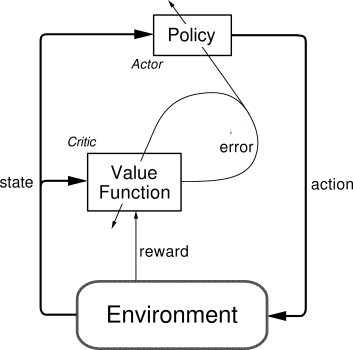
\includegraphics[width=200]{img/actor_critic.png}
\end{center}
\caption[Actor Critic diagram]
{Representation of the Actor Critic interface.}
\label{fig:AC}
\end{figure}

In Figure \ref{fig:AC} you can see how the error is computed based on the approximation of the value function
changing how actor and critic behave.
The hole learning process depend on the error and is defined as the difference between the future returns and
the approximation of this value made by the algorithm.
More formally:
\begin{equation}
    \delta_t=r_{t+1}+\gamma V(s_{t+1})-V(s_t)
\end{equation}
By minimizing this error $\delta_t$ the policy will trend to the optimal policy.
The value function will also approximate more precisely future return values.


\subsection{\aclp{SMDP}\label{subsec:SMDP}}

A \ac{SMDP} is a framework for \newconcept{hierarchical reinforcement learning} in which actions are not atomic, in the sense that they
do not last for just one time step, can be composed by several smaller actions and make decisions based on several states.
%TODO CAMBIAR BETA AQUI O EN EL PARAMETRO DEL A3C SINO PUEDE SER CONFUSO

This complex actions are named options and can be expressed as a tuple $\langle \mathcal{I}, \pi, \beta \rangle$ where
$\mathcal{I}$ is the set of initial states
in which the option is available, $\pi$ is the policy that defines which actions must be taken inside the option and $\beta$ is a
probability distribution over states of the option being interrupted.
More formally, a Markov option is made up by:
\begin{itemize}
    \item $\mathcal{I} \subseteq \mathcal{S}$ where $\mathcal{S}$ is the set of states
    \item $\pi : \mathcal{S} \times \mathcal{A} \rightarrow [0,1]$ where $\mathcal{A}$ is the set of available actions
    during the option, it can also contain other options.
    \item $\beta : \mathcal{S} \rightarrow [0,1]$
\end{itemize}
Since an option can be composed by several actions or other options, and each action lasts one time step, an
option may last more time steps.

%TODO QUITAR ESTO SI NO LO USO
With Markov options the interrupt decision is made on the current state $s_t$ but sometimes we may want to end an option if
some specific amount of time has elapsed.
For this purpose semi-Markov options were created, they use the history of
states and actions taken in that option to select the next action and the end condition.
So in both $\pi$ and $\beta$ instead of
using $\mathcal{S}$ it uses $\Omega$ which is the set of all histories $h_{t\tau}$ defined as follows:
\begin{equation}
    h_{t\tau} = \{s_t,a_t,r_{t+1},s_{t+1},a_{t+1}, ..., r_\tau, s_\tau\}
\end{equation}
Where $\tau$ is the holding time of the option, thus is, the amount of time steps it takes to complete.
Finally the three components of a semi-Markov option are:
$\pi : \Omega \times \mathcal{A} \rightarrow [0,1]$, $ \beta : \Omega \rightarrow [0,1]$ and
$\mathcal{I} \subseteq \mathcal{S}$

A \ac{SMDP} is a variation of an \ac{MDP} where the set of actions $\mathcal{A}_s$ is made up by semi-Markov options.
A \ac{SMDP} problem can be expressed as a tuple $\left< \mathcal{S}, \mathcal{O}_s, P_o(s,s'), R_o(s),\gamma \right>$ where:
\begin{itemize}
    \item $\mathcal{S}$ is the state space
    \item $\mathcal{O}_s$ is the set of possible options available in state $s$.
    \item $P_o(s,s')$  is the likelihood of reaching state $s' \in \mathcal{S}$ from state $s \in \mathcal{S}$ when taking
    option $o \in \mathcal{O}_s$, discounted depending on the time taken to reach it.
    \begin{equation}
        P_o(s,s') = \sum_{k=1}^\infty p(s', k) \gamma^k
    \end{equation}
    Where $p(s',k)$ is the probability that the option $o$ terminates in $s'$ after $k$ steps.
    \item $R_o(s)$ is the expected reward for taking option $o$ in state $s$.
    To define it we must introduce $\varepsilon(o,s,t)$ which denotes the event of $o$ being initiated in state $s$ at time $t$.
    \begin{equation}
        R_o(s) = E\left\{ r_{t+1} + \gamma r_{t+2} + \gamma^2 r_{t+3} + \dots
        + \gamma^{k-1} r_{t+k} \;|\; \varepsilon(o,s,t)\right\}
    \end{equation}
    \item $\gamma \in [0,1]$ is the discount factor.
\end{itemize}

With \acp{SMDP} we can define multiple levels of agents where, for example, some of them control basic actions and others
complex options.

\section{\aclp{ANN}}
In this section we describe what are \acfp{ANN},
how they work and which are the most important variants for this thesis.
Most of the definitions and figures are taken from \citetitle{simon2009NN}
by \citet{simon2009NN}

An \ac{ANN} is a collection of artificial neurons that process information in a
parallel way and stores experiential knowledge to use it in another experiences.
It continually adapts connexions between neurons to reach some goals, this process
is named learning.

\subsection{Artificial neuron}
An \newconcept{artificial neuron}, from now on called \newconcept{neuron}, is an
information-processing unit modeled as a mathematical
function with these five basic elements:
\begin{itemize}
    \item A set of connecting links with some weight associated.
    A signal $x_j$ at the input of connexion $j$ related to neuron $k$ is multiplied by the weight $w_{kj}$.
    \item An adder for summing the weighted input signals.
    \item An activation function $\varphi(\cdot)$ that limits the amplitude of the output of a neuron.
    \item A bias $b_k$ which has the effect of increases or reduces the input of the activation function.
    \item An output signal $y_k$ which is the result of the processed information.
\end{itemize}

\begin{figure}[hbtp]
\begin{center}
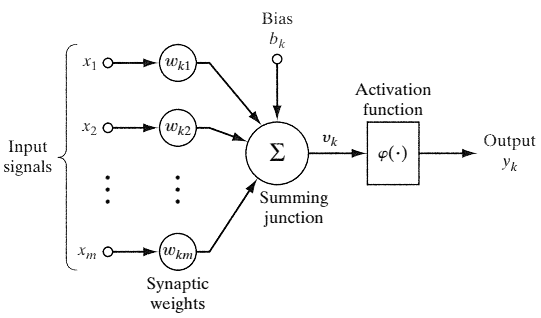
\includegraphics[width=300]{img/artificial_neuron.png}
\end{center}
\caption[Artificial neuron diagram]
{Achitecture of an artificial neuron}
\label{fig:AN}
\end{figure}

In mathematical terms we describe the neuron with the following equation:
\begin{equation}
    y_k=\varphi(b_k+\sum\limits_{j=1}^m w_{kj} x_j)
\end{equation}
where $x_1, x_2, \dots, x_m$ are the input signals;
$w_{k1}, w_{k2}, \dots, wk_m$ are the respective weights of neuron $k$;
$b_k$ is the bias;
$\varphi(\cdot)$ is the activation function;
and $y_k$ is the output signal of the neuron.

\subsection{Multilayer perceptron}
A \newconcept{multilayer perceptron} is a kind of ANN made up by several ordered \newconcept{layers} of neurons.
It is characterized by having an input layer, several hidden layers and an output layer.

The input layer is a set of neurons whose inputs are not connected to other neurons and whose outputs are connected to
the first hidden layer.
Each of the hidden layers satisfies that the output of neurons in layer $i$ is the input of some neurons in layer $i+1$,
except the last hidden layer that is connected with the output layer.
The output layer is a set of neurons whose results form the output signal of the network.
When each neuron has as input all neurons of previous layer the network is named fully connected.

\begin{figure}[hbtp]
\begin{center}
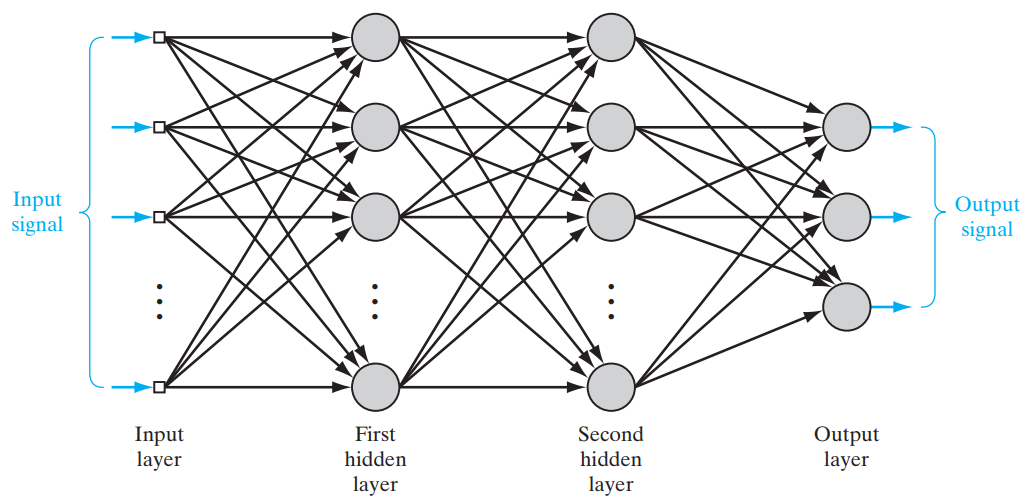
\includegraphics[width=400]{img/multilayer_perceptron.png}
\end{center}
\caption[Multilayer perceptron diagram]
{Fully connected multilayer perceptron.}
\label{fig:FullyMP}
\end{figure}

In multilayer perceptrons there are two kinds of signals, \newconcept{function signals} and \newconcept{error signals}.

A function signal is an input signal that propagates through the network generating an output signal.
The output signal is the result of the function parametrized by all the weights and biases of all neurons.

An error signal originates at the output layer and propagates backwards through the network.
It approximates the difference between the output signal and the desired output signal, given that we are using the \ac{ANN}
to approximate some function.
Each node computes its contribution to the error by estimating the gradient with respect its weights and bias.

The process of adjusting the weights and biases of each neuron to approximate a required output signal given some input
signal is named \newconcept{training}.

Fully connected layers are the most computationally expensive to train because of the amount of connexions and variables.
One way of reducing complexity is to use \newconcept{shared weights}, instead of having different weights for each input of each neuron,
some part of the weights of a neuron are reused to be multiplied for the input of another neurons.
This reduces the number of variables the network should maintain and update, but the number of mathematical computations
will be the same.

Another way of reducing the number of computations is by reducing the number of nodes.
\newconcept{Pooling layers} do that, is a form of non-linear downsampling that applies a function to a group of nodes resuming them
in just one node.

\subsection{Transfer learning in \aclp{ANN} \label{subsec:TransferLearning}}
The aim of \newconcept{transfer learning} techniques is to improve the learning process of a new task, given some previous knowledge
about related tasks.
Neural networks, especially the deepest ones, need tons of data to adjust their weights to successfully perform some tasks.

A way to reduce the amount of training data needed and speed up the learning process is to reuse some \ac{ANN} previously
trained for a similar task.
Then the \ac{ANN} adapts its weights to succeed in the target task.
For example, if we want to recognize dogs inside images, we could use some existing \ac{ANN} developed to recognize cats and
then adapt its weights.

Another method is to train our network in a general problem related to the target task to later focus on it.
With \acfl{DNN} we could train a large network on some task and then reuse just the first layers, that should
contain a basic feature extraction about the problem.
In the previous example we could take the layers of the network responsible of recognizing shapes and add some new nodes
to train on recognizing dogs.
A simpler example is to train the full network first to recognize shapes and then train on dogs.

\section{\acl{DL}}
\acf{DL} is a machine learning method based on high-level representations of the data.
It basically extends \acp{ANN} by adding multiple hidden layers creating huge neural networks with lots of parameters and interrelations.

In the last years this technique has become really popular as a consequence of its great results comparing to human level performance in many tasks.

\subsection{\acl{CNN} \label{subsec:CNN}}

This network is a variation of the multilayer perceptron specifically designed to recognize visual patterns.
They are usually made up of four different types of layers: \newconcept{convolutional layers}, \newconcept{\acfl{ReLU} layers},
\newconcept{pooling layers} and fully connected layers.

Convolutional layers apply a convolution to some previous layer, characterized by a filter.
Each node defines its connections based on the filter and their position. The filter is made up by \newconcept{kernel size},
\newconcept{stride}, \newconcept{padding} and \newconcept{values}.
The kernel size defines the shape and amount of nodes of the previous layer that are connected to a convolutional layer node.
The stride defines how the kernel moves across the previous layer, with each move, the filter is applied to some group of
nodes by connecting them to a new node of the convolutional layer.
The padding (specifically zero padding) is the amount of zeros to add around the border of each dimension in the previous
layer, this helps to preserve as much information about the previous layer values.
Finally, the values define the weights for each input signal in each neuron.
These are the same values for each convolutional layer node.
This concept is named \newconcept{shared weights} and minimizes the amount
of variables the neural network has to retain and update.

\ac{ReLU} layers increases the nonlinear properties of the model by applying the function $f(x)=max(0,x)$ to all outputs of the previous layer.
It is common practice to apply this layer after convolutional layers.
Applying \ac{ReLU} functions mitigates the \newconcept{vanishing gradient problem}, which is characterized of an exponential
reduction of the gradient through the layers.

Pooling layers generate a downsampled version of the previous layer.
It applies some function ( usually a max function ) to a group of outputs of the previous layer and saves the result in
just one node of the pooling layer.
This technique reduces the parameters of the network which decrease the memory and calculations needed, it also reduces overfitting.

\subsection{\acl{DQN}}
This algorithm was introduced by \citeauthor{mnih2015human} in \citetitle{mnih2015human} (\citeyear{mnih2015human}).

A \acl{DQN}, from now on \ac{DQN}, is a deep convolutional neural network designed to approximate Q values of reinforcement learning.
This agent learns from images to approximate the optimal action-value function (\ffref{subsec:Qlearn}).
The aim of \acp{DQN} is to learn successful policies directly from images of some given problem, for example, a game.
For that purpose the output of the network will be the Q values of each action given some input state.

Bear in mind that when using \acp{ANN} in reinforcement learning the learning problem can become unstable or even diverge.
This is caused by the weight updates, that changes not only the result of som action-value pair but all of the action-value associations;
the correlation present in sequence of observations;
and the correlations between the action-values and target values.
For that reason, apart from the \ac{ANN}, they used an experience replay ($E$).
This structure saves last $T$ states which the environment has gone by in the format $e_t=(s_t, a_t, r_t, s_{t+1})$.
Then it picks in an uniformly random manner from this set to train the network.
Training on independent and identically distributed samples helps reducing the instability generated by the neural network.

Q-learning updates are organized in iterations, containing several training steps.
Each iteration has its fixed network
parameters $\theta^-_i$ and applies several training steps obtained from the experience replay to finally change them.
This updates are characterized by the loss applied to the network to adjust its weights.
They defined the loss function in the following way:
\begin{equation}
    L_i(\theta_i)=E_{(s,a,r,s') \sim U(D))} \left [ \bigg(r+\gamma \max_{a'}Q(s',a';\theta_i^-)-Q(s,a;\theta_i)\bigg )^2\right ]
\end{equation}
Where $\theta_i$ and $\theta^-_i$ are the wights of two neural networks with the same architecture.
$\theta_i$ is updated each training step while $\theta^-_i$ only change when the iteration finish, following
$\theta_i = \theta^-_i$ after this happens.

This network has successfully surpass human-level skills in many Atari games.
But in Montezuma's Revenge it was unable to obtain any score (see \ffref{subsec:MontezumasRevenge}).

\subsection{\acl{A3C}\label{subsec:A3C}}
The algorithm \acl{A3C}, from now on \ac{A3C}, was introduced by \citeauthor{mnih2016A3C} in
\citetitle{mnih2016A3C} (\citeyear{mnih2016A3C}).

The main difference between asynchronous methods and the methodology used in \ac{DQN} is the experience replay.
In \ac{A3C} instead of having an experience replay, to take uniformly random states and avoid instability, it runs in
parallel multiple instances of the environment.
At each time step the agent is being trained with different states of multiple environments that runs in isolation.

Another difference between \ac{DQN} and \ac{A3C} is the reinforcement learning approach.
It uses the actor-critic interface introduced in \ffref{subsec:AC}.
It defines two \acp{ANN} that represent the value of the state ($V$) and the policy ($\pi$).
$V$ is the output of just one node, but $\pi$ is the output of a set of nodes, each one representing the probability of taking
an action.
In practice this two \acp{ANN} share almost all the layers, except the last one ($V$ and $\pi$).

%TODO A LO MEJOR HAY QUE DEFINIR N-STEP RETURNS EN ESE APARTADO
Also the loss function used to train the network differ from \ac{DQN}, it uses n-step returns (\ffref{subsec:returns}) and it does not
update $Q$ values, it updates $V$ and $\pi$.
The number of steps used in the loss function is $t_{max}$ ( an hyperparameter ) but if a
final state is reached before that, the loss is computed with less than $t_{max}$.
It also adds an entropy factor $H$ based on the policy, in order to improve exploration by discouraging premature
convergence to suboptimal deterministic policies.
\ac{A3C} uses the following update function:
\begin{equation}
    \nabla_{\theta'}\;log\:\pi(a_t\mid s_t;\theta')\;A(s_t,a_t;\theta,\theta_v)+\beta\nabla_{\theta'}H(\pi(s_t;\theta'))
\end{equation}
Where $A$ is the advantage function of n-step returns in terms of $V$.
$\theta'$ are the weights related to the policy and $\theta_v$ the weights related to the value function.
$\beta$ is an hyperparameter that controls the strength of the entropy regularization term.
The advantage function defines at follows:
\begin{equation}
    A_t=\sum^{k-1}_{i=0}\gamma^i r_{t+i}+\gamma^k V(s_{t+k};\theta_v)-V(s_t;\theta_v)
\end{equation}
Where $k$ can vary from state to state ( if a final state is reached ) and is upper-bounded by $t_{max}$.

This algorithm is parallelized in different threads which contain different replicas of a shared \ac{ANN}.
Each thread interacts with the environment using his own \ac{ANN}, until $t_{max}$ or end of game are reached, and updates the
global network parameters with the update function above.
The algorithm used in each thread is the following.

\begin{algorithm}[hbtp]
\begin{algorithmic}
    \State \newconcept{//Assume global shared parameter vectors $\theta$ and $\theta_v$ and global shared counter $T = 0$}
    \State \newconcept{//Assume thread-specific parameter vectors $\theta' and \theta_v'$}
    \State Initialize thread step counter $t \leftarrow 1$
    \Repeat
        \State Reset gradients: $d\theta \leftarrow 0$ and $d\theta_v \leftarrow 0$.
        \State Synchronize thread-specific parameters $\theta' = \theta$ and $\theta_v' = \theta_v$
        \State $t_{start} = t$
        \State Get state $s_t$
        \Repeat
            \State Perform $a_t$ according to policy $\pi(a_t|s_t;\theta')$
            \State Receive reward $r_t$ and new state $s_{t+1}$
            \State $t \leftarrow t + 1$
            \State $T \leftarrow T + 1$
        \Until{terminal $s_t $ \textbf{or} $t-t_{start} == t_{max}$ }
        \State R = \begin{cases}
                0,   & \text{ for terminal }\ s_t \\
                V(s_t, \theta_v'),   & \text{for non-terminal } s_t \;\newconcept{// Bootstrap from last state}\\
            \end{cases}
        \For{ $i \in \{ t-1,\dots,t_{start}\}$}
            \State $R \leftarrow r_i + \gamma R$
            \State Accumulate gradients wrt $\theta': d\theta \leftarrow d\theta + \nabla_{\theta'} log\:\pi(a_i\mid s_i;\theta')(R-V(s_i;\theta_v'))+\beta\nabla_{\theta'}H(\pi(s_i;\theta'))$
            \State Accumulate gradients wrt $\theta_v': d\theta_v \leftarrow d\theta_v + \partial(R-V(s_i;\theta_v'))^2 / \partial \theta_{v}'$
        \EndFor
        \State Perform asynchronous update of $\theta$ using $d\theta$ and of $\theta_v$ using $d\theta_v$.
    \Until{$T > T_{max}$}
\end{algorithmic}
\caption{\acl{A3C} - psudocode for each actor-learner thread (\cite{mnih2016A3C})}
\label{alg:A3C}
\end{algorithm}


%%% Local Variables:
%%% mode: latex
%%% TeX-master: "../report"
%%% End:
